% \documentclass[10pt]{sosp2015}
\documentclass[10pt,onecolumn]{sosp2015}
%\documentclass[10pt,twocolumn,letterpaper]{article}
%\usepackage[10pt,inchmargins]{sigmin}  %% template from Xi Wang.
%\special{papersize=8.5in,11in}
%\setlength{\pdfpagewidth}{8.5in}
%\setlength{\pdfpageheight}{11in}
% \usepackage[noheadfoot,
%             left=1in,right=1in,top=1in,bottom=1in,
%             columnsep=0.3in
%             ]{geometry}
\usepackage[small,compact]{titlesec}
\usepackage[font={small,bf}]{caption}    % added 9/10/13
\usepackage[nolineno,noindent,norules]{lgrind}
\usepackage{tightenum}
\usepackage{float}
\usepackage{xspace}
\usepackage{times,pifont}
\usepackage{mathptmx}
\usepackage{subfig,graphics,graphicx,color}
\usepackage{multirow}
\usepackage{dblfloatfix} %% correctly orders single- and double-col figures
\usepackage{hyphenat}
\usepackage{mathrsfs}
\usepackage{subfig}
\usepackage{amssymb,amsmath,centernot}
\usepackage{lastpage}
\usepackage{flushend}
\usepackage{hhline}
\usepackage{authblk}
%\newcommand{\doi}{XXXXXX}


%%% ================= START of SOSP '13 template ================= 
% \makeatletter
% 
% \def\ftype@copyrightbox{8}
% \def\@copyrightspace{
% \@float{copyrightbox}[b]
% \begin{center}
% \setlength{\unitlength}{1pc}
% \begin{picture}(20,6.0) 
% \put(0,3){\parbox{\columnwidth}{\scriptsize
% 
% %*** SAMPLE. AUTHOR PUT SUPPLIED TEXT HERE ****
% 
% \noindent
% \rule{6.0 cm}{0.2pt}\\
% Permissiondddd to make digital or hard copies of part or all of this work 
% for personal or classroom use is granted without fee provided that
% copies are not made or distributed for profit or commercial advantage 
% and that copies bear this notice and the full citation on the first
% page. Copyrights for third-party components of this work must be
% honored.  For all other uses, contact the Owner/Author. 
% 
% \vspace{\baselineskip}\noindent
% Copyright is held by the Owner/Author(s).\\
% \textit{SOSP'15}.\\
% ACM XXXXXXX.
% 
% \noindent
% http://dx.doi.org/\doi}
% }
% \end{picture}
% \end{center}
% \end@float}
% 
% \def\maketitle{\par
%  \begingroup
%    \def\thefootnote{\fnsymbol{footnote}}
%    \def\@makefnmark{\hbox
%        to 0pt{$^{\@thefnmark}$\hss}}
%      \twocolumn[\@maketitle]
% \@thanks
%  \endgroup
%  \setcounter{footnote}{0}
%  \let\maketitle\relax
%  \let\@maketitle\relax
%  \gdef\@thanks{}\gdef\@author{}\gdef\@title{}\gdef\@subtitle{}\let\thanks\relax
%  \@copyrightspace}
% 
% \makeatother

%%% ================= END of SOSP '13 template ================= 



%\newcommand{\comment}[1]{}
\frenchspacing

%\doublespacing

%%%%%%%%%%%%%%%%%%%%%%%%%%%%
%     macro

\newcommand{\xxx}[0]{\textsc{Crane}\xspace}
\newcommand{\paxos}[0]{\textsc{Paxos}\xspace}
\newcommand{\mytitle}[0]{\textbf {\paxos Made Transparent}}
\newcommand{\mykeywords}[0]{State Machine Replication, Fault Tolerance, Stable 
and Deterministic Multithreading, Software Reliability}

%%%%%%%%%%%%%%%%%%%%%%%%%%%%%%%%%%%%%%%%%%%%%%%%%%%%%%%%%%%%%%%%%
% hyperref stuff

%\usepackage[square,comma,numbers,sort]{natbib}
\usepackage{hypernat}
\usepackage{hyperref}

%% fill in pdf info here
\hypersetup{%
colorlinks=false,
pdfborder={0 0 0},
pdftitle={\mytitle},
pdfkeywords={\mykeywords},
bookmarksnumbered,
pdfstartview={FitH},
urlcolor=cyan,
pdfpagelabels=true,
pdfdisplaydoctitle=true,
}%

%\usepackage{breakurl}
%\usepackage[all]{hypcap}
%\renewcommand{\url}{\burl}

%%%%%%%%%%%%%%%%%%%%%%%%%%%%%%%%%%%%%%%%%%%%%%%%%%%%%%%%%%%%
% Some NICE fonts

\newfont{\BIG}{cminch}                             %--- One-inch font
\newfont{\sfbHuge}{cmssbx10 scaled\magstep5}       %-- 25pt sans serif bold
\newfont{\sfbLarger}{cmssbx10 scaled\magstep3}   %-- 12+pt sans serif boldd
\newfont{\sfblarger}{cmssbx10 scaled\magstep2}   %-- 12+pt sans serif bold
\newfont{\sfblarge}{cmssbx10 scaled\magstep1}      %-- 12pt sans serif bold
\newfont{\sfbeleven}{cmssbx10 scaled\magstephalf}  %-- 11pt sans serif bold
\newfont{\sfb}{cmssbx10}                           %-- 10pt sans serif bold
\newfont{\sfeight}{cmss8}                          %-- 8pt sans serif

%%%%%%%%%%%%%%%%%%%%%%%%
%    space tweaking

%\textwidth = 6.5 in
%\textheight = 9.0 in
%\setlength{\topmargin}{-.5in}

%\headheight = 0.0 in
%\headsep = 0.0 in
%\parskip = 0.2in
%\parindent = 0.0in

\renewcommand{\topfraction}{0.95}
\addtolength{\textfloatsep}{-0.1in}
%\addtolength{\floatsep}{0.025in}
\renewcommand\floatpagefraction{.9}
%\renewcommand\bottomfraction{.9}
\renewcommand\textfraction{.1}

\setlength{\parindent}{9pt}

% Rescue
\makeatletter
\def\v#1{{\mbox{\fontfamily{cmtt}\fontsize{\f@size}{\f@size}\selectfont #1}}}

\newcommand{\dmt}[0]{DMT\xspace}
\newcommand{\smt}[0]{StableMT\xspace}
\newcommand{\smr}[0]{SMR\xspace}

\newcommand{\racepro}[0]{\textsc{RacePro}\xspace}
\newcommand{\criu}[0]{\textsc{CRIU}\xspace}
\newcommand{\lxc}[0]{\textsc{LXC}\xspace}
\newcommand{\tern}[0]{\textsc{Tern}\xspace}
\newcommand{\peregrine}[0]{\textsc{Peregrine}\xspace}
\newcommand{\parrot}[0]{\textsc{Parrot}\xspace}
\newcommand{\repframe}[0]{\textsc{RepFrame}\xspace}
\newcommand{\grace}[0]{Grace\xspace}
\newcommand{\coredet}[0]{\textsc{CoreDet}\xspace}
\newcommand{\kendo}[0]{Kendo\xspace}
\newcommand{\dthreads}[0]{\textsc{DThreads}\xspace}
\newcommand{\determinator}[0]{Determinator\xspace}
\newcommand{\dos}[0]{dOS\xspace}
\newcommand{\ddos}[0]{DDOS\xspace}
\newcommand{\timealgo}[0]{time bubbling\xspace}
\newcommand{\ldpreload}[0]{LD\_PRELOAD\xspace}
\newcommand{\ntimeout}[0]{$W_{timeout}$\xspace}
\newcommand{\nclock}[0]{$N_{clock}$\xspace}

\newcommand{\apache}{\v{Apache}\xspace}
\newcommand{\mongoose}[0]{\v{Mongoose}\xspace}
\newcommand{\ab}{\v{ApacheBench}\xspace}
\newcommand{\clamav}{\v{ClamAV}\xspace}
\newcommand{\upnp}{uPnP\xspace}
\newcommand{\mediatomb}{\v{MediaTomb}\xspace}
\newcommand{\mencoder}{\v{mencoder}\xspace}
\newcommand{\mongodb}{\v{MongoDB}\xspace}
\newcommand{\ssdb}{\v{SSDB}\xspace}
\newcommand{\mysql}{\v{MySQL}\xspace}
\newcommand{\sysbench}{\v{SysBench}\xspace}
\newcommand{\zookeeper}{\v{ZooKeeper}\xspace}


\newcommand{\aget}[0]{\v{aget}\xspace}
\newcommand{\pthread}[0]{\mbox{Pthreads}\xspace}
\newcommand{\openldap}[0]{{OpenLDAP}\xspace}
\newcommand{\redis}[0]{{Redis}\xspace}
\newcommand{\bdb}[0]{{Berkeley DB}\xspace}
\newcommand{\vtune}[0]{\v{VTune}\xspace}
\newcommand{\http}[0]{\mbox{HTTP}\xspace}

% In short.
\newcommand{\eg}{{e.g.}}
\newcommand{\ie}{{i.e.}}
\newcommand{\etc}{{etc}}
\newcommand{\para}[1]{\vspace{.00in}\noindent{\bf #1}}
\newcommand{\wrt}{{w.r.t. }}
\newcommand{\cf}{{cf. }}

% Synch and network operations.
\newcommand{\checktimebubble}[0]{\v{check\_add\_timebubble()}\xspace}
\newcommand{\mutexlock}[0]{\v{pthread\_mutex\_lock()}\xspace}
\newcommand{\connect}[0]{\v{connect()}\xspace}
\newcommand{\send}[0]{\v{send()}\xspace}
\newcommand{\sendto}[0]{\v{sendto()}\xspace}
\newcommand{\sendmsg}[0]{\v{sendmsg()}\xspace}
\newcommand{\mywrite}[0]{\v{write()}\xspace}
\newcommand{\pwrite}[0]{\v{pwrite()}\xspace}
\newcommand{\close}[0]{\v{close()}\xspace}
\newcommand{\recv}[0]{\v{recv()}\xspace}
\newcommand{\select}[0]{\v{select()}\xspace}
\newcommand{\poll}[0]{\v{poll()}\xspace}
\newcommand{\epollwait}[0]{\v{epoll\_wait()}\xspace}
\newcommand{\accept}[0]{\v{accept()}\xspace}

% Parrot primitives.
\newcommand{\getturn}[0]{\v{get\_turn()}\xspace}
\newcommand{\putturn}[0]{\v{put\_turn()}\xspace}
\newcommand{\wait}[0]{\v{wait()}\xspace}
\newcommand{\signal}[0]{\v{signal()}\xspace}

% Evaluation stats.
\newcommand{\github}[0]{\url{github.com/columbia/crane}}
% \newcommand{\ntype}[0]{four\xspace}
\newcommand{\nprog}[0]{five\xspace}
\newcommand{\overheadmax}[0]{22.99\%\xspace}
\newcommand{\overhead}[0]{34.19\%\xspace}
\newcommand{\dmtspeedup}[0]{10.5\%\xspace}
\newcommand{\proxyoverhead}[0]{2.33\%\xspace}
\newcommand{\timebubblelow}[0]{66.65\%\xspace}
\newcommand{\timebubblehigh}[0]{93.88\%\xspace}
\newcommand{\recovertime}[0]{1.97ms\xspace}
\newcommand{\downgradetime}[0]{0.36s\xspace}
\newcommand{\mencoderspeedup}{\v{49\%}\xspace}

\def\LGfsize{\footnotesize}
%\pagestyle{empty}


\conferenceinfo{SOSP'15}{October 4--7, 2015, Monterey, CA}
\copyrightyear{2015} 
\copyrightdata{978-1-4503-3834-9/15/10} 
\doi{2815400.2815427}

\title{\mytitle}
% \authorinfo{Heming Cui, Rui Gu, Cheng Liu, Tianyu Chen, Junfeng Yang}{The 
% University of Hong Kong, Columbia University}

\author[+*]{Heming Cui}
\author[*]{Rui Gu}
\author[*]{Cheng Liu}
\author[x]{Tianyu Chen}
\author[*]{Junfeng Yang}
\setlength{\affilsep}{0.5em}
\renewcommand\AB@affilsepx{\hspace{28.0 mm}\protect\Affilfont}
\affil[+]{\textrm\fontsize{10}{10}\selectfont The University of Hong Kong}
\affil[*]{\textrm Columbia University}
\affil[x]{\textrm Tsinghua University\vspace{-7.0 mm}}

\begin{document}

% Hack for: Package caption Error: No float type 'copyrightbox' defined.
%\newcounter{copyrightbox}

\date{}

%\author[+]{\hspace{0 mm}\fontsize{10}{10}\selectfont Paper 247, SOSP 2015}
\maketitle
%\thispagestyle{empty}

\begin{sloppypar}
\begin{abstract}
State machine replication (\smr) leverages distributed consensus protocols
such as \paxos to keep multiple replicas of a program consistent in face
of replica failures or network partitions.  This fault tolerance is
enticing on implementing a principled SMR system that replicates general
programs, especially server programs that demand high
availability. Unfortunately, \smr assumes deterministic execution, but
most server programs are multithreaded and thus nondeterministic.
Moreover, existing \smr systems provide narrow state machine interfaces to
suit specific programs, and it can be quite strenuous and error-prone to
orchestrate a general program into these interfaces

We have built \xxx, an \smr system that transparently replicates
general server programs. \xxx achieves distributed consensus on the socket
API, a common interface to almost all server programs.  It leverages \parrot,
a deterministic multithreading system we built, to make multithreaded replicas 
deterministic. It uses a new technique we call \emph{time bubbling} to 
efficiently tackle a difficult challenge of nondeterministic network input 
timing. Evaluation on \nprog widely used server programs (\eg, \apache, 
\clamav, and \mysql) shows that \xxx is easy to use, has moderate overhead, and 
is robust. \xxx has the potential to grealty improve the reliability and 
availability of general programs. \xxx's source code is at \github.

\end{abstract}
\end{sloppypar}

% \begin{sloppypar}
%% %\category{D.2.5}{Software Engineering}{Testing and Debugging}
%% \category{D.4.5}{Operating Systems}{Threads, Reliability}
%% \category{D.2.4}{Software Engineering}{Software/Program Verification}
%% \terms{Algorithms, Design, Reliability, Performance}
%% \keywords{\mykeywords}

%% \vskip 2mm
%% \noindent {\small \bf Categories and Subject Descriptors:} \vskip -.2mm
%% \noindent
%% {\footnotesize D.4.5~[{\bf Operating Systems}]: {Threads, Reliability}\\
%% D.2.4~[{\bf Software Engineering}]: {Software/Program Verification};}
%% \vskip 1mm
%% \noindent {\small \bf General Terms:} \vskip -.2mm
%% \noindent
%% {\footnotesize Algorithms, Design, Reliability, Performance}
%% \vskip 1mm
%% \noindent {\small \bf Keywords:} \vskip -.2mm
%% \noindent
%% {\footnotesize \mykeywords}

% \vskip 2mm
% \noindent {\small \bf Categories and Subject Descriptors:}
% {\small D.4.5~[{\bf Operating Systems}]: {Threads, Reliability};
%   D.2.4~[{\bf Software Engineering}]: {Software/Program Verification};}
% \vskip .1mm
% \noindent {\small \bf General Terms:} {\small Algorithms, Design,
%   Reliability, Performance}
% \vskip .1mm
% \noindent {\small \bf Keywords:} {\small \mykeywords}
% 
% \end{sloppypar}

%%%%%%%%%%%%%%%%%%%%%%%%%%%%%%%%%%%
% Add page number.
\setcounter{page}{1}
\pagenumbering{arabic}

\thispagestyle{plain}
\pagestyle{plain}
\setlength{\footskip}{20pt}
%%%%%%%%%%%%%%%%%%%%%%%%%%%%%%%%%%%

\begin{sloppypar}

\vskip 2mm
\noindent {\small \bf Categories and Subject Descriptors:}
{\small D.4.5~[{\bf Operating Systems}]: {Threads, Reliability};
  C.2.4~[{\bf Computer-communication Networks}]: {Distributed Systems};}
\vskip .1mm
\noindent {\small \bf General Terms:} {\small Algorithms, Design,
  Reliability, Performance}
\vskip .1mm
\noindent {\small \bf Keywords:} {\small \mykeywords}

\end{sloppypar}

\begin{sloppypar}

\section{Introduction} \label{sec:intro}

\emph{State machine replication (\smr)} models a program as a deterministic 
state machine, where the states are important program data and the transitions 
are deterministic executions of program code under input requests.  \smr runs 
replicas of the program and invokes a distributed consensus protocol (typically 
\paxos~\cite{paxos,paxos:simple,paxos:complex}) to ensure the same sequence of 
input requests for replicas, as long as a quorum (typically a majority) of the 
replicas agrees on the input request sequence. Under the deterministic execution 
assumption, this quorum of replicas must reach the same exact state despite 
replica failures or network partitions.  \smr is proven safe in 
theory and provides high availability in 
practice~\cite{paxos:live,paxos:practical,chubby:osdi,paxos:datastore, 
bolosky:nsdi11,mencius:osdi08,eve:osdi12,rex:eurosys14}.

The fault-tolerant benefit of \smr makes it particularly attractive on 
implementing a principled replication system for general programs, especially 
server programs that require high availability.  Unfortunately, doing so remains
quite challenging; the core difficulty lies in the deterministic state
machine abstraction required by \smr, elaborated below.

First, the deterministic execution assumption breaks down in today's
server programs because they are almost universally multithreaded. Even on the 
same exact sequence of input requests, different executions of the same exact 
multithreaded program may run into different thread interleavings, or 
\emph{schedules}, depending on such factors as OS scheduling and physical 
arrival times of requests. Thus, they can easily exercise different schedules 
and reach divergent execution states -- a difficult problem well recognized by 
the community~\cite{dos:osdi10,eve:osdi12,ddos:asplos13,rex:eurosys14}.
To tackle this problem, one prior approach,
execute-verify~\cite{eve:osdi12}, detects divergence of execution states
and retries, but it relies on developers to manually annotate states, a
strenuous and error-prone process.

Second, to leverage existing \smr systems such as
ZooKeeper~\cite{zookeeper}, developers often have to shoehorn their
programs into the narrowly defined state machine interfaces provided by
these \smr systems.  Ideally, experts -- those with intimate knowledge of
the arcane (think how many 
papers~\cite{paxos,paxos:simple,paxos:complex,paxos:live,paxos:practical} are 
needed to explain \paxos),
under-specified~\cite{paxos:practical} \smr protocols and subtle failure
scenarios in distributed systems -- should build a solid \smr system,
which all other developers then leverage. However, an \smr system often
has to settle for a specific state and transitional interface because it
cannot anticipate all possibilities in which developers structure their
programs.  For example, Chubby~\cite{chubby:osdi} defines a lock server
interface, and ZooKeeper a pseudo file system interface.  Orchestrating a
sever program into such a narrow interface not only requires
intrusive and error-prone modifications to the program's structure and
code, but also disrupts the \smr system itself at times. For instance,
developers abused Chubby for storage~\cite{chubby:osdi}, causing the
Chubby developers to add quota support.

We present \xxx,\footnote{\xxx stands for Correctly ReplicAting
  Nondeterministic Executions. It is also our hope that our system is as
  elegant as the identically named bird.} an \smr system that
transparently replicates server programs for high availability.  With
\xxx, a developer focuses on implementing her program's intended
functionality, not replication.  When she is ready to replicate her
program for availability, she simply runs \xxx with her program on
multiple replicas.  Within each replica, \xxx interposes on the socket and
the thread synchronization interfaces to keep replicas in sync.
Specifically, it considers each incoming socket call (\eg, \accept a
client's connection or \recv a client's data) an input request, and
runs a \paxos consensus protocol~\cite{paxos:practical} to ensure that a
quorum of the replicas sees the same exact sequence of the incoming socket calls.


To address nondeterminism, we have built three \emph{deterministic 
multithreading (\dmt)} systems~\cite{cui:tern:osdi10, peregrine:sosp11, 
parrot:sosp13}. \dmt~\cite{dpj:oopsla09,dmp:asplos09,kendo:asplos09,
coredet:asplos10, 
dos:osdi10,ddos:asplos13,ics:oopsla13} typically maintains a \emph{logical 
time}\footnote{Though related, the logical time in \dmt is not to 
be confused with the logical time in distributed systems~\cite{lamportclock}.} 
that advances deterministically on each thread's synchronization. By 
serializing thread synchronizations, \dmt practically makes an entire 
multithreaded execution deterministic. The overhead of \dmt is typically 
moderate because most code is not synchronization and can still run in parallel. 
Specifically, \xxx leverages \parrot~\cite{parrot:sosp13}, our latest \dmt 
system. \parrot incurs merely 12.7\% overhead in 
average on a wide range of 108 popular multithreaded programs on 24-core 
machines.

A key challenge on realizing \smr for multithreaded executions is that,
simply combining \paxos and \dmt is not sufficient to keep replicas in
sync, because the physical time that each request arrives at different
replicas may still be different, easily leading to divergence of execution
states and outputs.

Two prior approaches attempted to tackle this challenge.  
Execute-agree-follow~\cite{rex:eurosys14} records a partially
ordered schedule of \pthread synchronizations on one replica and replays it 
on the other replicas, which may incur high network bandwidth 
consumption and performance overhead. dOS~\cite{dos:osdi10} also leverages
\dmt for replication, but it determines the logical admission time for
each request using two-phase commit.  Aside from two-phase commit's known
intolerance of primary failures, per-request commit is also costly.

One may consider solving this challenge by leveraging the underlying
distributed consensus protocol to determine the logical admission time for each
request.  Specifically, when running the consensus protocol to decide each
request's position in the request sequence, a predicted logical admission time 
can be carried as part of the decision as well. Unfortunately, 
predicting a logical admission time for each request accurately is quite 
challenging because typical server programs have background threads which 
may frequently tick logical clocks. A too-small predication leads to 
replica divergence if another replica has already run past the predicted 
logical time. A too-large predication blocks the system unnecessarily 
because replicas cannot admit the request before reaching the predicted time.

Our key insight is that many requests need no admission time consensus
because their admission times are already deterministic.  Hypothetically,
if the requests arrive faster than they are admitted at each replica, each
request's admission time is fully deterministic because each replica
simply admits requests as fast as it can. In practice, requests do not arrive 
this fast.  However, there are still frequent bursts of requests that arrive 
together. Among replicas, as long as the first request of a burst is admitted at 
a deterministic logical time, all the other requests in the burst are admitted 
at deterministic logical times without requiring consensus.

Leveraging this insight, we created an technique called \emph{\timealgo} to 
enforce deterministic logical times efficiently.  It ensures that the 
first request in a burst is admitted at each replica deterministically by 
inserting a deterministic wait after the previous burst of requests are all 
admitted.  During this wait, each replica only processes already admitted 
requests, and does not admit new requests.  \xxx negotiates a consistent 
duration of the wait via the underlying distributed consensus protocol, and 
enforces this wait at each replica via \dmt.  These waits are like 
deterministic time bubbles between bursts of requests (hence the name of the 
technique), creating the illusion that the requests arrive faster than they are 
admitted.

In short, by converting per-request admission time consensus to per-burst,
\timealgo efficiently combines the input determinism of \paxos and the
execution determinism of \dmt.  For busy servers, requests in bursts
greatly outnumber the other requests.  (We observed that \timebubblelow to
\timebubblehigh of requests are in bursts; see \S\ref{sec:overhead}.) They
rarely need to invoke time consensus, enjoying good performance.  For idle
servers, time consensus overhead does not matter much because the servers
are idle anyway.



% P10: Evaluation highlights.
We implemented \xxx by interposing on the POSIX socket and the \pthread
synchronization interfaces.  It intercepts operations along these
interfaces by hijacking dynamically linked library calls for transparency.
It implements the \paxos protocol atop libevent~\cite{libevent} for
distributed consensus, and leverages our \parrot system for deterministic
multithreading.  Unlike prior \smr systems with narrow interfaces, \xxx's
checkpoint and recovery must work with general programs. To this end, it
leverages \criu~\cite{criu} to checkpoint and restore process states, and
\lxc~\cite{lxc} for file system states.  An additional benefit of using
the \lxc container is that \xxx isolates the replicated server program
from the environment, avoiding nondeterministic systems resource contentions.


We evaluated \xxx on \nprog widely used server programs,
including \http servers \apache and \mongoose, an anti-virus server
\clamav, a \upnp multimedia server \mediatomb, and a database server \mysql. 
Our results on popular performance benchmarks show that \xxx works with
all the servers easily (three servers require no modification, and the
other two servers each require only two lines of \parrot hints~\cite{parrot:sosp13}
to improve performance); that \xxx's performance overhead is
moderate (an average of \overhead overhead at the servers' peak 
performance setups on our 24-core machines); and that \xxx is robust on replica 
failures.

In the remainder of this report, \S\ref{sec:overview} introduces \xxx's 
architecture and assumptions. \S\ref{sec:eval} presents evaluation results. 
\S\ref{sec:conclusion} concludes, and \S\ref{sec:recommendation} presents 
recommendations.




























% % \section{Background} \label{sec:background}
% This section first introduces \paxos, the core of typical \smr systems; and 
% then describes Determinsitic Multithreading (\dmt), a recent advanced technique 
% that eliminates nondeterminism and enforces the same schedule for a 
% multithreaded program on the same input; and then we briefly introduce how users 
% use our \xxx system.
% 
% \subsection{The \paxos Consensus Protocol} \label{sec:paxos}
% TBD.
% 
% \subsection{Deterministic Multithreading} \label{sec:dmt}
% TBD.

\section{\xxx Overview} \label{sec:overview}

\xxx is deployed as a typical \smr system. A set of three or five replicas is 
set up within a LAN, and each replica runs an \xxx instance containing the 
same server program. On the \xxx system starts, one replica becomes the 
\emph{primary} (or leader) replica which proposes the order of requests to 
execute, and the others become backup replicas which follow the primary's 
proposals. A number of clients in LAN or WAN send network requests 
to the primary and get responses.  If the primary machine fails, the other 
replicas run a leader election (\S\ref{sec:paxos}) to elect a new primary.

This section first presents \xxx's architecture, including its consensus 
interface and a \xxx instance's main components, and then uses an 
example to show how \xxx works with server programs.

% \subsection{Usage} \label{sec:usage}
% TBD.

\subsection{Architecture} \label{sec:abstraction}

To support general server programs transparently, \xxx chooses the POSIX socket 
API as its consensus interface. \xxx enforces two kinds of orders for socket
calls. First, for client programs' out going socket calls (\eg, \connect and
\send), \xxx enforces that all replicas see the same sequence of client socket 
calls with \paxos. \xxx does not need to order the clients' 
blocking socket calls because \xxx is not designed to replicate clients. 
Second, for a server program's blocking socket calls (\eg, \poll, \accept, and 
\recv), \xxx enforces that these calls are scheduled and 
returned in the same sequence of logical times across replicas. \xxx 
responses to the clients only using the server program on the primary, and it 
drops the responses of the server programs on backups.

For a server program's outgoing socket calls (\eg, \send), \xxx simply 
schedules them using \dmt and does not invoke consensus. The 
reason is that these calls readily have consistent contents via enforcing 
the same logical admission times of input requests and the same thread 
schedules for server programs across replicas.

\begin{figure}[t]
\centering
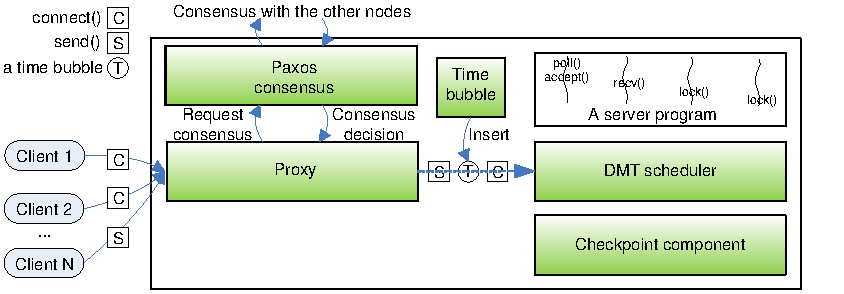
\includegraphics[width=.5\textwidth]{figures/repbox}
\vspace{-.20in}
\caption{{\em The \xxx Architecture.} \xxx components are shaded (and in
  green).} \label{fig:repbox}
\vspace{-.05in}
\end{figure}

Figure~\ref{fig:repbox} shows a \xxx instance running on the primary. The 
instance contains five main components, the proxy, the 
\paxos consensus, the \dmt scheduler, the \timealgo component that enforces the 
same logical clocks for servers' blocking socket calls across
replicas via inserting time bubbles, and the checkpoint component that 
periodically checkpoints the server program. A server program runs 
transparently in a \xxx instance without being aware of \xxx's components. A 
backup replica runs the same \xxx instance except that its proxy does not 
accept connections from clients and does not invoke consensus.

%% Each component.
The proxy component is a \xxx instance's gateway.  It accepts socket
requests from clients and forwards the requests to the server program on its 
own replica. It accepts responses from the server program and forwards the 
responses to the clients. Once the proxy receives a
client socket request, it invokes the \paxos consensus component running
on its own replica for this request.  The proxy does not block-wait for 
this decision which may take a while to reach. Once the proxy is notified by 
the \paxos component that some requests' decisions are made, it forwards the 
requests in decision order to the server program.

% Only the primary's proxy receives requests from the clients and initiates the 
% consensus process, but every proxy forwards requests to the server program on 
% its own replica.

The \paxos consensus component is a \paxos protocol that receives a client 
socket request from its own proxy and invokes a consensus process on
this request.  This component is also the only \xxx component that
communicates among different replicas. \xxx's \paxos implementation is 
based on a well-known and concise protocol~\cite{paxos:practical}. More
details on our \paxos implementation are given in \S\ref{sec:paxos}. After
\xxx's \paxos components reach consensus on a client socket call, each \paxos 
component notifies its own proxy to forward this call to its server program.

The \dmt component runs within the server program's process. \xxx leverages 
\parrot~\cite{parrot:sosp13} as the \dmt scheduler because \parrot 
runs fast on a wide range of 108 popular multithreaded programs. Specifically, 
\parrot uses a runtime technique called \ldpreload to dynamically intercept 
\pthread synchronizations (\eg, \mutexlock) issued by an executable and 
enforces a well-define, round-robin schedule on these synchronization 
operations for all threads, practically eliminating nondeterminism in thread 
synchronizations.

Although \parrot is not designed to resolve data races
deterministically, \xxx's replication tolerates data races that have
fail-stop consequences, and can further catch the
other data races by running a race detector on a backup replica (see
\S\ref{sec:limit}).  \xxx augments the \dmt component to schedule the
return points of socket calls in server replicas, too, to ensure that
requests are admitted at consistent logical times across replicas.

The \timealgo component sits between the proxy and the \dmt's processes, and it 
is invoked on two conditions. First, on a server's bootstraps, \xxx invokes 
time bubble insertions to make sure that the server programs across replicas 
reach the same initial state and wait for the first input request. Second, if 
the \dmt component has not received any input request from the proxy for a 
physical duration \ntimeout, a time bubble insertion is invoked as the boundary 
of two request bursts. To ensure the same sequence of inserted time bubbles 
across replicas, the same \paxos consensus as that for client socket calls is 
invoked. For each time bubble, each replica's \dmt scheduler promises to run a 
number of \nclock synchronizations and not to admit any 
client socket call.

If the \dmt scheduler exhausts the logical clocks in a time bubble, it either 
admits new client socket call (if any) or inserts another time bubble. If the 
scheduler does not exhaust the logical clocks after serving current requests, 
\parrot has a mechanism to exhaust them rapidly (\S\ref{sec:parrot}). More 
details on the \timealgo technique are given in \S\ref{sec:time-bubble}, and 
discussions on the values of the two parameters \ntimeout and \nclock are given 
in \S\ref{sec:sensitivity}.

% Across different runs of the \xxx system, this physical 
% duration may cause different number of inserted time bubbles; within the same 
% run, \xxx uses \paxos to preserve the same number of inserted time bubbles 
% across different replicas.



To recover from replica failures or add new replicas, the checkpoint 
component is invoked every minute on a backup replica. It
checkpoints the server process running with \dmt.  While one can always start a 
server replica from scratch and replay the entire sequence of socket calls, 
this replay can be extremely time-consuming for long-running servers.  Prior 
\smr systems rely on narrow state machine interfaces for checkpoint and
recovery, which does not work for general server programs. Instead, \xxx
leverages two popular open source tools: \criu, to checkpoint process 
state such as CPU registers and memory; and \lxc, to checkpoint the file 
system state of a server program's current working directory and installation 
directory.

Each checkpoint in \xxx is associated with a global index in \paxos's consensus 
order, so if one replica needs recovery, \xxx ships the latest checkpoint from a 
backup replica, restores the process running \dmt and the server program, and 
re-executes socket calls starting from this index. The proxy and consensus 
components do not require checkpoints because we explicitly designed their 
execution states independent to the server's process (\S\ref{sec:checkpoint}).

%% Overall guarantee. But go high level.


\subsection{Example} \label{sec:example}

\begin{figure}[t]
\centering
\begin{minipage}{.5\textwidth}
\lgrindfile{code/example.cpp.lineno}
\end{minipage}
\vspace{-.1in}
\caption{{\em A server example based on \apache.}} \label{fig:example}
\vspace{-.20in}
\end{figure}

\begin{figure}[t]
\centering
\begin{minipage}{.5\textwidth}
\lgrindfile{code/client.cpp.lineno}
\end{minipage}
\vspace{-.1in}
\caption{{\em A client example based on \v{curl}.}} \label{fig:client}
\vspace{-.05in}
\end{figure}

%TBD. Overall intro on the code.
Figure~\ref{fig:example} shows an example based on the \apache \http server. For 
clarity, the example uses worklist synchronization, and the actual servers use 
\pthread mutex locks and conditional variables which \xxx readily handles. The 
main thread creates a listener thread to accept client requests and a number 
of worker threads to process client requests in parallel. The listener listens 
on a port with \poll. When a new client connection comes, the 
listener calls \accept and appends the accepted socket descriptor to a 
worklist. Each worker thread blocks on a \v{worklist.get()} function until 
the worklist is not empty. It then dequeues an accepted socket, processes the 
request with a mutex lock acquired, and then sends a response. 
Figure~\ref{fig:client} shows an example based on client programs such as 
\v{curl}. This client connects to the server, sends one \http request, waits for 
the server's response, and then closes the connection.

Let's say a \xxx system with three replicas is set up, and each replica runs 
this server; two clients start simultaneously, and each sends a \http PUT 
and GET request respectively on the same URL ``a.php" to the primary.



\begin{figure}[t]
\centering
\begin{minipage}{.5\textwidth}
\lgrindfile{code/diff-sync-order.cpp}
\end{minipage}
\vspace{-.1in}
\caption{{\em HTTP GET request got the valid page due to the two requests' 
large arrival interval.}} \label{fig:yes-page}
\vspace{-.2in}
\end{figure}

\begin{figure}[t]
\centering
\begin{minipage}{.5\textwidth}
\lgrindfile{code/diff2-sync-order.cpp}
\end{minipage}
\vspace{-.1in}
\caption{{\em HTTP GET request didn't get the page due to the two requests'
small arrival interval.}} \label{fig:no-page}
\vspace{-.05in}
\end{figure}


% If for example
% there are multiple such clients sending POST requests simultaneously, the
% order in which the requests are processed can lead to different server
% states.

This server has three major sources of nondeterminism, 
which can easily cause its execution states across 
replicas to diverge. The first source (for short, $S_1$) is that clients' 
requests may arrive at different replicas in different orders. Second ($S_2$), 
within the server, the nondeterministic \pthread synchronizations may easily 
lead to different schedules. For instance, the \v{worklist.add()} called by 
the listener may wake up any worker blocking on \v{worklist.get()}.

Third ($S_3$), even if clients' requests arrive at different replicas in the 
same order, the physical time interval of each two consecutive requests can 
still be largely different across replicas depending on each request's physical 
arrival time. This variance may cause client socket calls to be 
admitted at inconsistent logical clocks across replica and lead to divergent 
execution states.

For instance, Figure~\ref{fig:yes-page} and Figure~\ref{fig:no-page} show two 
replicas' schedules, and each is a total order of executed socket calls or 
\pthread synchronizations in workers. Although the PUT and 
GET requests arrive at the two replicas in the same order, these requests' 
interval in the first schedule (Figure~\ref{fig:yes-page}) is much larger than 
that in the second one, causing the first one to return a page and the second 
one ``404 Not Found".

% even one 
% can always enforce that the PUT request arrives before the GET request, because 
% worker 2's \recv call in Figure~\ref{fig:yes-page} returns much later than that 
% in Figure~\ref{fig:no-page} (the line numbers in these figures can be viewed as 
% logical times), two different schedules and thus different outputs may show up.

% Worse, 
% the workers' \v{process\_req()} functions contain extra \pthread 
% synchronizations, then the server's blocking socket operations can return at 
% arbitrary logical points which interleave nondeterministically with these 
% synchronizations, easily leading to different schedules and execution states 
% across machines.

\begin{figure}[t]
\centering
\lgrindfile{code/paxos-queue-order.cpp}
\vspace{-.2in}
\caption{{\em A sequence of client socket calls enforced by 
\xxx.}}\label{fig:paxos-queue}
\vspace{-.25in}
\end{figure}

\begin{figure}[t]
\centering
\lgrindfile{code/example-sync-order.cpp}
\vspace{-.2in}
\caption{{\em A schedule of the server example enforced by 
\xxx across replicas.}}\label{fig:dmt-schedule}
\vspace{-.05in}
\end{figure}


\xxx works as follows. First, depending on the order the primary's proxy 
receives these requests, \xxx eliminates $S_1$ with \paxos and ensures the 
same request sequence for all replicas. Second, \xxx's \dmt 
scheduler eliminates $S_2$ by ensuring a deterministic order of \pthread 
synchronizations.

Third, depending on the time intervals of client socket calls 
observed by the primary, \xxx eliminates $S_3$ by dividing this sequence of 
calls into bursts with time bubbles. Figure~\ref{fig:paxos-queue} shows a 
sequence. Let's say the primary observes that the 
intervals of the \connect and \send calls are all smaller than \ntimeout, and 
the interval between the \send at Line 4 and the \close at Line 6 in the 
sequence is larger than \ntimeout. Then, \xxx inserts a time bubble at Line 5 
and divides the sequence into two bursts. For the calls in the first burst, all 
replicas admit them as is using \dmt even if some of their time intervals are 
larger than \ntimeout on some backups, consistently maintaining the logical 
admission times for these calls.

For the time bubble in this sequence, all replicas' \dmt schedulers promise to 
do only \nclock \pthread synchronizations and then admit a client 
socket call, consistently maintaining the logical admission times 
for the \close calls. Given this sequence, Figure~\ref{fig:dmt-schedule} shows 
\xxx's consistent schedule and output ``404 Not Found" across replicas. 
We ran \xxx with \apache and used \v{curl} to spawn concurrent PUT 
and GET requests, and we observed that \apache's network outputs were 
consistent across replicas (\S\ref{sec:correctness}).

In addition to enforcing consistency, the \timealgo technique is 
also efficient because it does per-burst consensus instead of per-request 
consensus. In this example, if more \connect calls arrive simultaneously and 
each client connection does more \send calls, the ratio of inserted 
time bubbles versus the total number of socket calls in the sequence may be 
even lower, then \xxx may become more efficient. Evaluation on popular servers 
and workloads shows that this ratio is often low and that \xxx has moderate 
overhead  (\S\ref{sec:overhead}).

% according to the primary's physical duration check on 
% \ntimeout, \xxx eliminates $S_3$ by inserting time bubbles which divide the 
% client requests into bursts. For the socket calls within each burst, \xxx's \dmt 
% schedulers consistently admit these calls as is regardless of the differences of 
% each call's physical arrival times across replicas. For each time bubble, \xxx's 
% \dmt schedulers across replicas promise to tick \nclock \pthread 
% synchronizations and not to admit any client socket call before then.



% KEY: Explain why there is such order fo client requests, and why there must be 
% A timebubble. Also explain the 100us boundary. Also, justified by experiments. 
% Also explain subsequent timebubbles may also be inserted.


% Enforcing logical admission times across replicas for the these socket calls 
% consistently is challenging. Consider the \close calls, on 
% the client side, the clients won't execute \close until the server sends 
% responses. On the server side, the server's worker threads keep executing 
% \pthread synchronizations and ticking \dmt's logical clocks. From a \dmt 
% scheduler's view, the clients' \close are external inputs and may be appended 
% to each replica's sequence at indefinite physical times. Therefore, these calls 
% and further socket calls may be admitted by the \dmt schedulers across 
% replicas at inconsistent logical clocks.

% In short, \xxx must ensure that these 
% \close calls are admitted by the \dmt schedulers across replicas at consistent 
% logical times.

% To tackle this challenge, \xxx inserts a time bubble at Line 5 of the sequence 
% to divide the client socket calls into two bursts. For each time bubble, the 
% \dmt scheduler promises to schedule exactly \nclock thread synchronizations and 
% not to admit any client socket call before then. If the server needs to execute 
% more \pthread synchronizations to process requests so that responses can be 
% sent and clients' \close calls can come, \xxx inserts more time bubbles. If 
% there are leftover clocks in a time bubble, \parrot, \xxx's \dmt scheduler, has 
% a mechanism to exhaust these clocks rapidly (\S\ref{sec:parrot}).

% KEY: explain why we did not need a time bubble for each request.
% In addition to addressing the consistency challenge, the \timealgo technique is 
% also efficient because it does per-burst consensus instead of per-request 
% consensus. From this example we can see that per-request consensus is 
% unnecessary because once the server's \accept calls return, the clients can do 
% \send calls immediately, making clients' \connect and \send come in one burst. 
% If more client \connect calls come simultaneously and each connection does more 
% \send calls, the ratio of inserted time bubbles vesus the total number of 
% socket calls in the sequence may be even lower, then \xxx may become more 
% efficient. Evaluation on popular servers and workloads confirmed that 
% this ratio is often low (\S\ref{sec:overhead}).


% KEY: change description: since incoming sequence is ready, timebubbles are 
% ready, so \dmt just schedules them as is. Three types of operations: regular 
% sync, blocking socket calls, and outgoing socket calls. Third, 
% Figure~\ref{fig:schedule}. 
% Given the sequence in Figure~\ref{fig:paxos-queue}, the \dmt scheduler's task 
% becomes easy. It pops the first client socket call in the sequence and 
% schedules a server thread blocking on a matching socket call. 
% For instance, \dmt schedules a server thread blocking on a \recv with a 
% matching \send in the sequence. If the \dmt scheduler sees a time bubble at 
% sequence head, it decreases this bubble's logical clock by one and does a 
% \pthread synchronization or a outgoing socket call (\eg, \send in Line 22 in 
% Figure~\ref{fig:example}). When the time bubble has no clock left, \dmt pops it 
% and postpones to schedule any synchronization until the next time bubble or 
% client socket call comes. If the primary's \dmt scheduler sees no client socket 
% call comes after postponing for a physical duration \ntimeout, it invokes a 
% \paxos consensus on ``inserting a time bubble" (\S\ref{sec:time-bubble}). 



% Let's say \xxx's primary sees that the \connect and \send calls 
% come in almost the same physical time, and it sees that the \close calls 
% come after the \send calls later than the physical duration \ntimeout.
% Figure~\ref{fig:paxos-queue} shows a sequence of the two 
% clients' outgoing socket calls and a time bubble inserted by \xxx. Because the 
% primary sees that the two \send calls come closely, it groups 
% these calls within the same burst. Then, even if the second \send call reaches 
% the other backups much later than the first \send call, \xxx consistently 
% treats the two \send calls as one burst across replicas. To match these two 
% \send calls, \xxx schedules the two \recv calls one next to the other at Line 9 
% and 10 in Figure~\ref{fig:dmt-schedule}, ensuring consistent logical clocks for 
% these \recv calls across replicas.
% 
% In addition, because the primary inserts a time bubble at Line 5 in 
% Figure~\ref{fig:paxos-queue}, all replicas consistently handle this time bubble 
% by ticking \nclock logical clocks and then admit the two \close calls, ensuring 
% consistent logical clocks for these two \close calls across replicas. 




% However, in real-world, the clients' socket operations do not come in one
% single burst. The reasons can be network congestion causing a delay, or
% the clients just waiting for the server's responses.  For example, our
% client program waits for a response from the server before it closes the
% connections.  When the \paxos socket request queue is empty and one of the
% threads wants to do a blocking network operation, the \dmt component
% cannot just block the thread and let other threads run until the next
% request arrives.  If it does so, the next request will most likely be
% admitted at different logical times across replicas because replicas run
% and advance their logical times at different speeds.  The \dmt component
% cannot just block all threads, either, because there are requests being
% processed and the next request may lag indefinitely.  

% To address this timing issue, we have created a new technique called
% \timealgo.  The \dmt scheduler waits for a short amount of time, and if
% the queue is still empty, \dmt requests the proxy to insert a time bubble
% to the queue which contains a fixed amount of logical clocks. The primary
% node's proxy asks for consensus on a time bubble insertion into the \paxos
% queue. After replicas reach consensus on this insertion, each machine's
% \dmt scheduler can tick the same amount of logical clocks in this time
% bubble to process already admitted requests and send responses to
% clients. More time bubbles will be inserted if necessary. If there are
% leftover clocks in a time bubble, when new requests come, the \dmt
% scheduler \xxx leverages invokes an \emph{idle thread} mechanism
% (\S~\ref{sec:parrot}) to quickly consume these clocks consistently across
% machines and process new requests.

% Figure~\ref{fig:paxos-queue} shows a sequence of client socket operations with 
% a time bubble \xxx inserts. By enforcing this same sequence across different 
% machines, \xxx enforces the same sequence of logical clocks and thus the same 
% resultant schedules across different machines, as shown in 
% Figure~\ref{fig:dmt-schedule}.

 


% When the primary fails and a new primary is elected, clients need a way to
% connect to the new primary or transparently migrate their existing
% connections to the new primary.  We assume some standard fail-over
% DNS/networking techniques in place for this purpose as in existing
% replication systems.

% %\section{Interface} \label{sec:example}
%TBD.
% \section{\xxx's Synchronization Wrappers for a Server} \label{sec:wrappers}

This section describes how \xxx handles a server program's 
synchronizations, including \pthread synchronizations and blocking socket 
calls. Because how to handle these synchronizations is tightly relevant 
to the \parrot \dmt scheduler we leverage, in this section, we first introduce 
some background on the \parrot scheduler, including its primitives and wrappers. 
And then we describe how \xxx leverages \parrot's primitives and wrappers to 
implement its own synchronization wrappers.

\subsection{Background: the \parrot Scheduler} \label{sec:parrot}

\begin{figure}[t]
\centering
\begin{minipage}{.5\textwidth}
\lgrindfile{code/dmt-interface.cpp}
\end{minipage}
\vspace{-.1in}
\caption{{\em The \parrot \dmt runtime's scheduler primitives.}} 
\label{fig:dmt-primitives}
\vspace{-.05in}
\end{figure}

\parrot~\cite{parrot:sosp13} is a \dmt system that uses the \ldpreload trick to 
intercept \pthread synchronizations at runtime and enforces a 
well-define, round-robin order for these operations. In this round-robin 
manner, \parrot first lets one runnable thread do one synchronization 
operation; and then, for the left runnable threads, \parrot lets the next 
thread do one synchronization operation; and then the next runnable thread, 
until all runnable threads having done one synchronization operation. Then 
\parrot repeats. To enforce this schedule, \parrot maintains a queue of runnable 
threads (\emph{run queue}) and another queue of waiting threads (\emph{wait 
queue}), like a Linux OS scheduler.

\parrot enforces an important invariant: only the thread at the head of the run 
queue can do one actual synchronization operation and manipulate the run queue 
and wait queue. After the head thread does one operation, it rotates itself 
to the tail of the run queue and wakes up the new head thread of the run queue. 
Conceptually, threads within \parrot pass a global token (the run queue head) 
around. A thread will be put into the wait queue if the synchronization object 
it requires is not available, and it will be put back to the run queue 
when this object becomes available.

\begin{figure}[t]
\centering
\begin{minipage}{.5\textwidth}
\lgrindfile{code/lock.cpp.lineno}
\end{minipage}
\vspace{-.1in}
\caption{{\em \parrot's wrapper for \mutexlock.}} 
\label{fig:lock}
% \vspace{-.05in}
\end{figure}

To implement this round-robin schedule in a compact way, \parrot provides a 
monitor-like internal interface, shown in Figure~\ref{fig:dmt-primitives}. The 
\getturn function waits until the calling thread becomes the head of the run 
queue. The \putturn function rotates the calling thread to the tail of the run 
queue and wakes up the next thread which now is the head of the run queue. The 
\wait function puts the calling thread from run queue to wait queue and blocks 
on a opaque object (\eg, a mutex or a socket descriptor), until another 
thread makes this object available and calls a \signal on this object. When a 
thread returns from a \wait function, it becomes the head of the run queue. 
Both the \wait and the \signal functions require getting the global turn.

These set of primitives are highly optimized for multi-core. Each thread has an 
integer flag and condition variable. The \getturn function spin-waits on the 
current thread's flag for a while before blocking on the condition variable. 
The \wait function needs to get the turn before it returns, so it uses the same 
combined spin- and block- wait strategy as the \getturn function. The \getturn 
and \signal functions signal both the flag and the conditional variable of the 
next thread. In common case, these operations acquire no lock and do not 
block-wait, thus the number of synchronization context switches in \parrot is 
much smaller than that in traditional \pthread synchronizations, yielding 
faster performance in \parrot than in the \pthread runtime for some 
programs~\cite{parrot:sosp13}.

% For instance, \parrot's evaluation~\cite{parrot:sosp13} showed that, when 
% transcoding an OSDI 2012 presentation video using a popular parallel transcoder 
% \mencoder, \parrot only incurred 921 context switches, while the traditional 
% Linux \pthread runtime incurred 1.9M context switches, leading to a 
% \mencoderspeedup speedup of \mencoder with \parrot.

Figure~\ref{fig:lock} shows the \mutexlock wrapper in \parrot. This wrapper 
uses try-lock to avoid deadlock: if the head of the run queue is blocked waiting 
for a lock before giving up the turn, no other thread can get the turn.

When all threads of a program block, which is common case in a server 
program, \parrot puts an internal \emph{idle thread} to the run queue, which 
simply does repetitive \getturn and \putturn operations. This idle thread 
ensures that \parrot's run queue always has threads and that \parrot's logical 
clock keeps ticking.

\parrot's blocking socket calls are nondeterministic because it 
is a \dmt system for eliminating nondeterminism in \pthread 
synchronizations. A blocking socket call's wrapper in \parrot works as 
follows. When a thread calls a blocking socket call, the thread 
calls \getturn, passes the global token to the next thread in the run 
queue, removes itself from the run queue, and then calls into the 
actual socket call. When the thread returns from the actual call, it appends 
itself to a \emph{socket queue}. Each thread at the run queue head moves the 
threads in this socket queue back to the run queue. This move-back is 
nondeterministic because threads may return from blocking socket calls 
nondeterministically and thus may be added to the socket queue in various 
orders.
% However, \parrot's invariant, only the thread at run queue 
% head can manipulate the run queue, is maintained.

\subsection{\xxx' Synchronization Wrappers for a Server}
\label{sec:socket-wrappers}

\begin{figure}[t]
\centering
\begin{minipage}{.5\textwidth}
\lgrindfile{code/check-timebubble.cpp.lineno}
\end{minipage}
\vspace{-.1in}
\caption{{\em \xxx's \checktimebubble function.}} 
\label{fig:checktimebubble}
\vspace{-.10in}
\end{figure}

\xxx wraps a rich set of common blocking socket operations, including \select, 
\poll, \epollwait, \accept, and \recv. \xxx also modifies the wrappers of 
\pthread synchronizations. These wrappers are sufficient for the server 
programs in our evaluation.

% These wrappers enforce the same logical clocks for 
% server programs' blocking operations and \pthread synchronizations across 
% different replicas and do the actual synchronization operations.

\xxx needs to modify the \mutexlock wrapper in Figure~\ref{fig:lock} to do 
three things. First, if the \paxos request sequence has been empty for a 
physical duration \ntimeout, \xxx requests a time bubble with \nclock logical 
clocks. Second, if the head of the \paxos sequence is a time bubble, \xxx 
decreases the logical clock in the time bubble by one, or it removes this bubble 
if zero clock is left. Third, \xxx signals a thread that blocks on a socket 
operation (\eg, \recv) if there is a matching client socket call (\eg, \send) at 
the head of the \paxos sequence. To do these three things, \xxx calls the 
\checktimebubble function (defined in Figure~\ref{fig:checktimebubble}) at Line 
3 of the \mutexlock wrapper in Figure~\ref{fig:lock}.

An important data structure in \xxx's wrapper is the \paxos sequence which 
contains clients' socket calls and inserted time bubbles. This sequence sits 
between the proxy and the server's processes, and it is implemented with 
Boost~\cite{boost} shared memory. \xxx uses \v{lockf()} to ensure mutual 
exclusion on this sequence because the two processes may concurrently 
manipulate this sequence. For clarity, these lock and unlock operations are 
omitted in the pseudo code.

\begin{figure}[t]
\centering
\begin{minipage}{.5\textwidth}
\lgrindfile{code/recv.cpp.lineno}
\end{minipage}
\vspace{-.1in}
\caption{{\em \xxx's wrapper for \recv.}} 
\label{fig:recv}
\vspace{-.05in}
\end{figure}

\xxx also needs to modify \parrot's idle thread mechanism because sometimes 
this thread is the only thread in the run queue, and \xxx needs to frequently 
check whether a new client socket call comes or a time bubble insertion is 
needed. To do so, \xxx replaces \parrot's \getturn and \putturn primitives 
within the idle thread to be mutex lock and unlock operations, then the idle 
thread also runs the function defined in Figure~\ref{fig:checktimebubble} to 
check and insert time bubbles.

% Introduce the poll wrapper. This is tricky because instead of letting 
% Unlike \parrot, \xxx's blocking socket calls of a server program across 
% replicas can be scheduled at consistent logical times with the \paxos sequence 
% of client socket calls and the inserted time bubbles. 

Figure~\ref{fig:recv} shows \xxx's wrapper for the \recv call. This wrapper 
ensures that the \recv calls of server programs across replicas return at 
consistent logical times. The other blocking socket calls' wrappers are 
similar. A thread calling \recv in \xxx simply calls \getturn and blocks on the 
socket descriptor using \parrot's \wait primitive. When a client 
\send call that matches this \recv becomes the head of the \paxos sequence, 
the \mutexlock wrappers wakes up the server thread blocking on \recv with the
\signal call at Line 9 in Figure~\ref{fig:checktimebubble}. The waken up thread 
dequeues a number of matching \send calls from the \paxos sequence according to 
the actual bytes received. Also, for clarity, the lock and unlock operations for 
the \paxos sequence are omitted in this \recv wrapper.


\section{The Time Bubbling Technique} \label{sec:time-bubble}

\begin{figure}[t]
\centering
\includegraphics[width=.5\textwidth]{figures/time-bubble-flow}
\vspace{-.40in}
\caption{{\em The request and time bubble flow.}} \label{fig:bubbleflow}
\vspace{-.05in}
\end{figure}

Figure~\ref{fig:bubbleflow} shows the time bubbles inserted by the \timealgo 
technique. The technique groups clients' socket operations as bursts. A request 
burst can be a group of real socket requests (rectangles), or can be a time 
bubble with a fixed number of logical clocks (circles). In this figure, black 
requests are the first operation for each burst.


In a conceptual level, \xxx uses three rules to enforce the same sequence of 
logical times for socket requests (rectangles) and thus the same schedules 
across different replicas. First, \xxx uses \paxos to ensure the same 
sequence of client socket calls as well as inserted time bubbles as a 
``\paxos request sequence" for each replica, as shown in each horizontal arrow. 
Second, \xxx uses \dmt to guarantee that it only ticks logical clocks (\ie, 
schedules \pthread synchronizations or socket operations) when this 
sequence is not empty. Third, the \timealgo technique ensures that this 
sequence is not empty, otherwise it inserts a time bubble.


Figure~\ref{fig:handlebubble} shows the work flow of our \timealgo technique 
with four steps. Each replica's \dmt just waits for a physical duration 
\ntimeout, if no further requests come, (1) the \dmt requests its own proxy to 
insert a time bubble. (2) The proxy then checks whether it sees itself as the 
primary in the \paxos protocol. If so, it asks (3) the consensus component to 
invoke consensus on whether inserting this bubble; otherwise it drops this 
request. After a consensus on this bubble insertion is reached, (4) each 
machine's proxy simply inserts the bubble into the \paxos sequence, granting 
\nclock logical clocks to the \dmt scheduler.


If a server has not exhausted the logical clocks in a time bubble after 
serving current requests, \parrot's idle thread mechanism 
(\S\ref{sec:parrot}) exhausts these clocks rapidly. 
Then, the server can continue to process further requests in time.

\begin{figure}[t]
\centering
\includegraphics[width=.5\textwidth]{figures/handle-time-bubble}
\vspace{-.30in}
\caption{{\em The work flow of inserting a time bubble.}} 
\label{fig:handlebubble}
\vspace{-.1in}
\end{figure}

% Note that even given the same sequence of real socket operations, across 
% different executions, a server program running in \xxx may still run into 
% different schedules because \dmt only waits for a short amount of time (Line 5 
% in Figure~\ref{fig:lock}) and then requests time bubbles and a SIGUSR2 signal 
% across processes may get lost. However, across different machines, the servers 
% still run the same schedules because \paxos ensures that the same amount of 
% time bubbles as well as real socket requests for the \dmt schedulers across 
% replica nodes.



% \section{Implementation Details} \label{sec:impl}

\subsection{The \paxos Protocol} \label{sec:paxos}
The \paxos consensus component (\S\ref{sec:abstraction}) is a critical 
component to enforce a consistent total order of socket calls from client 
programs. Although there are already a number of open source \paxos 
implementations~\cite{concoord, zookeeper, libpaxos}, we re-implemented a \paxos 
protocol in order to incorporate our new socket-API consensus interface.

Our \paxos implementation is based on a well-known and concise 
approach~\cite{paxos:practical}. In normal case, only the primary invokes 
consensus, thus this approach reaches consensus efficiently. In exceptional 
cases such as primary restarts, a \paxos leader election 
is invoked to resolve conflicts. In \xxx, we implemented this election via 
making the primary send a heart beat message to all the backups every 
second, and if backup replicas have not receive any heart beat message for 
three seconds, these replicas start to elect a new leader. The 
leader election contains three steps~\cite{paxos:practical}: (1) backups 
proposing a new view, which is a standard \paxos two-phase 
consensus~\cite{paxos:simple}, (2) the proposer that wins the view proposing 
itself as a primary candidate, another standard \paxos two-phase consensus, and 
(3) the new leader announcing itself as the new primary.

In our implementation, each socket call from 
the client is assigned a global, monotonically increasing viewstamp (or 
\emph{global index}) to associate with each checkpoint 
(\S\ref{sec:checkpoint}). Upon consensus on a socket call, each consensus 
component persistently stores the call type, arguments, and global index into a 
Berkeley DB storage~\cite{berkeleydb} on SSD.

Although our current \paxos implementation focuses on supporting socket 
consensus interface, this \paxos protocol logic is independent of the types and 
arguments of socket operations, so our \paxos implementation can be applied 
to other types of consensus interface as well.

\subsection{Checkpoint and Restore} \label{sec:checkpoint}
To recover or add a new replica, \xxx leverages two popular open source 
tools: \criu~\cite{criu}, to checkpoint process state such as CPU registers and 
memory; and \lxc~\cite{lxc}, to checkpoint the file system state of a server 
program's current working directory and installation directory. These two 
directories are sufficient to capture files modified by the server programs in 
our evaluation.

Incorporating \lxc into \xxx has two extra practical benefits. First, the 
server process is ran within an \lxc, which provides the server the same 
and clean initial systems state and mitigates contentions on systems resources
(\eg, file descriptors) with other processes. Second, \lxc snapshots make \xxx 
easy to deploy on multiple replicas without worrying about slight differences of 
the systems environments such as kernel and library versions. We just built \xxx 
on one replica once, did a \lxc snapshot, and then copied the snapshot to 
other replicas.

A \xxx checkpoint operation contains three steps. First, \xxx 
uses \criu to checkpoint the server's process running within the \lxc 
container and dumps the checkpoint to the process's current working directory. 
\criu needs to modify systems files (\eg, ns\_last\_pid), but \lxc's 
default isolation configuration does not permit these modifications, so we 
configure \lxc to run in ``unconfined mode". Second, \xxx stops the container, 
uses ``\v{diff --text}" to generate a patch of current working directory and 
the server's installation directory against an \lxc snapshot prepared before 
any server starts. This file system checkpoint patch is incremental and 
thus efficient (\S\ref{sec:recovery}). Third, \xxx restarts the container, and 
restores the server process with \criu.

Such a \xxx checkpoint operation is done every minute on one 
backup replica without affecting the other replicas' performance. We 
explicitly design \xxx's proxy and consensus component stateless and they do not 
require checkpoints. A \xxx restore operation reverts these steps.

One main issue on checkpointing a server process is that it constantly accepts 
socket connections, but checkpointing and restoring 
TCP stacks are notoriously difficult. Our trick to avoid this difficulty is 
based on an observation: even busy server programs have some idle moments. For 
instance, consider \apache, even running with its standard performance-stress 
benchmark \ab, we observed that in some moments the server has no alive socket 
connections. Thus, during a checkpoint operation, \xxx simply checks whether the 
server has alive connections. If so, \xxx backs off for a few seconds and then 
retries until the server has no alive connections. Since checkpoint periods do 
not have to be precise, this trick runs well (\S\ref{sec:recovery}). 
% \section{Discussions} \label{sec:discussion}

This section first discusses \xxx's limitations and then introduces its 
applications.

\subsection{Limitation} \label{sec:limit}

% \xxx's key benefit is that a server program's blocking socket operations and 
% \pthread synchronization operations return at the same logical clocks across 
% different replicas, if a server program has no data race, no ad-hoc 
% synchronization, and does not have nondeterministic functions (\eg, 
% \v{rand()}).

\xxx leverages \parrot to make synchronizations deterministic.  \parrot is
explicitly designed not to handle data races. However, in the context of \xxx,
data races are less harmful because, if they cause backups to crash, \xxx
can still operate and recover as long as a quorum of the replicas is
still alive. Moreover, leveraging \xxx's replication architecture, one can 
deploy a race detector on a backup replica~\cite{repframe:apsys15}, achieving 
both good \xxx performance and full determinism.

There are other sources of nondeterminism besides thread scheduling and
request timing.  These other sources of nondeterminism may cause backups
to diverge, too.  For example, backups may do different things based on
their IP addresses, data read from \v{/dev/random}, addresses returned by
\v{malloc}, physical time observed via \v{gettimeofday}, or delivery time
of signals.  Prior work has shown how to eliminate these sources of
nondeterminism using record-replay~\cite{scribe:sigmetrics2010, 
respec:asplos10} or OS-level techniques~\cite{dos:osdi10}, which \xxx can 
leverage.  Another solution is to treat all these sources as inputs and 
leverage distributed consensus to let all replicas observe the same input.  We 
leave these ideas for future work. We inspected server 
programs' network outputs among replicas, and we found that these outputs 
were consistent in \xxx except physical times (\S\ref{sec:correctness}).

For a server program that spawns multiple processes which communicate via
IPC, \xxx currently does not make these IPC operations deterministic.  We
expect that it should be easy to support deterministic IPC in \xxx because it
already makes socket API deterministic.  In addition,
dOS~\cite{dos:osdi10} and DDOS~\cite{ddos:asplos13} have many effective
techniques for tackling this problem, which \xxx can leverage.

\subsection{Applications} \label{sec:app}

We envision three applications for \xxx. First, \xxx can 
be leveraged by other replication concepts (\eg, byzantine fault 
tolerance~\cite{pbft:osdi99, zyzzyva:sosp07}) 
and record-replay~\cite{scribe:sigmetrics10, racepro:sosp11, respec:asplos10} 
because they also suffer from nondeterminism. Second, promising 
results in \repframe~\cite{repframe:apsys15} have shown that \xxx's transparent 
replication architecture can enable multiple types of program analysis tools 
within one execution, making a server program enjoy benefits of multiple 
analyses. Third, \xxx's determinism as well as its \timealgo technique alone can 
be applied to mitigate timing channels~\cite{Askarov:ccs10, Zhang:ccs11, 
Aviram:ccsw10}.
\section{Evaluation} \label{sec:eval}

Our evaluation was done on a set of three replica machines, with each having 
Linux 3.13.0, 1Gbps bandwidth LAN, 2.80 GHz dual-socket hex-core Intel Xeon 
with 24 hyper-threading cores, 64GB memory, and 1TB SSD.

We evaluated \xxx on \nprog widely used server programs, 
including \http servers \apache~\cite{apache} and \mongoose~\cite{mongoose}; 
\clamav~\cite{clamav}, an anti-virus scanning 
server that scans files in parallel and deletes malicious ones; 
\mediatomb~\cite{mediatomb}, a \upnp multimedia server that uploads, shares, 
and transcodes pictures and videos in parallel; and \mysql~\cite{mysql}, an 
SQL database. Although \mysql has a replication 
feature~\cite{mysql:replication}, this feature is mainly for improving read 
performance, not for providing \smr fault tolerance.

\smr's high availability and fault-tolerance are attractive to these 
servers programs, because these programs provide on-line service and contain 
important in-memory execution states and storage (\eg, \clamav's 
security database, \mediatomb's SQLite~\cite{sqlite} database, and \mysql).

For \apache and \mongoose, we used \apache's own concurrency stress testing 
benchmark \ab to invoke concurrent \http requests for a PHP page, which takes 
about 70 ms for a PHP interpreter to generate the page contents. For \clamav, 
we used its own client utility \v{clamdscan} to request the server to scan 
\clamav's own source code and installation directories in parallel. For 
\mediatomb, because it has a web interface, we used \ab to invoke concurrent 
requests which use \mencoder~\cite{mencoder} to transcode a 15MB video from AVI 
to MP4. For \mysql, we used \sysbench~\cite{sysbench} to generate random select 
queries. These workloads triggered 8$\sim$12 threads in each server program to 
process requests concurrently at peak performance on our machines. These 
popular benchmarks and workloads cover CPU, network, and file-IO 
bounded operations.  

% , and they involve diverse blocking socket calls 
% (\eg, \poll, \select, \epollwait, \accept, and \recv) and intensive \pthread 
% synchronizations.

\xxx has two parameters for the \timealgo technique. The first 
parameter, $W_{timeout}$, is the physical duration that the primary's \dmt 
scheduler waits before it requests consensus on a time bubble insertion. To 
prevent this parameter significantly deferring responses, \xxx sets its 
default value 100us, two orders of magnitudes smaller than the workloads' 
response times and wide-area network latencies.

The second parameter, $N_{clock}$, is the number of logical 
clocks within each time bubble. \xxx sets its default value 1000, because we 
observed that the amounts of executed \pthread synchronizations to process each 
request in most of the evaluated servers are closed to this scale. We used 
these default values in all evaluations unless explicitly specified. A 
sensitivity evaluation on these two parameters showed that their default 
values were reasonable choices (\S\ref{sec:sensitivity}).

To mitigate network latency, benchmark clients were ran within 
the replicas' LAN. Larger latency will mask \xxx's overhead. We measured each 
workload's response time as it has direct impact on users. For each data 
point, we ran 1K requests for 20 times and then picked the median value.

The rest of this section focuses on these questions:

\begin{tightenum}

\item[\S\ref{sec:ease-of-use}:] Is \xxx easy to use?

\item[\S\ref{sec:correctness}:] Compared to nondeterministic executions, does 
\xxx consistently enforce the same sequence of network outputs among replicas?

\item[\S\ref{sec:overhead}:] What is \xxx's performance overhead compared to 
nondeterministic executions?

\item[\S\ref{sec:hint}:] When the default schedules enforced by the \parrot 
\dmt scheduler are slow, how much optimization can \parrot's performance hints 
bring to \xxx?

\item[\S\ref{sec:sensitivity}:] How sensitive are the two \timealgo parameters 
to \xxx's performance?

\item[\S\ref{sec:recovery}:] How fast are \xxx's checkpoint and recovery 
components on handling replica failures?

% \item[\S\ref{sec:race}:] If some \xxx users care about data races much, how 
% does \xxx tolerate the slowdown of data race detector by deploying it on a 
% replica?

% \item[\S\ref{sec:lesson}:] What practical lessons have we learnt during the 
% case study on these server programs with \xxx?

\end{tightenum}







\subsection{Ease of Use} \label{sec:ease-of-use}

All \nprog servers we evaluated were able to be transparently plugged and 
played in \xxx without modification. For \clamav, \mediatomb, and \mysql, we 
did not need to modify any line of code and they already have moderate 
performance overhead compared to the un-replicated nondeterministic executions. 
For \apache and \mongoose, the default schedules serialized parallel 
computations. For each of the two servers, we added two lines of soft barrier 
performance hints invented by \parrot~\cite{parrot:sosp13} to line up parallel 
computations as much as possible and compute efficient \dmt schedules (cf 
\S\ref{sec:hint}).

\subsection{Consistency of Network Outputs} \label{sec:correctness}

To verify whether the server programs running in different replicas maintain 
the same execution states, we compared each server program's network outputs 
logged in three replicas. Network outputs imply a server's execution states, 
including the outcomes of ad-hoc synchronizations and data races, which 
synchronization schedules can not capture. We ran the performance workloads and 
logged the order and contents of server programs' outgoing socket calls, 
including \send, \sendto, \sendmsg, \mywrite, and \pwrite. These calls are 
sufficient to capture all network outputs of the evaluated programs. We then 
used \v{diff} to compare the logs across replicas. 

We designed two experiment plans. In plan I, we ran \xxx with the 
programs. In plan II, we disabled only the \timealgo component in \xxx for 
three reasons: (1) we wanted to know whether \timealgo is needed to keep 
replicas in sync, (2) enabling \paxos made us easy to ship the same workload 
to replicas, and (3) enabling \parrot made us easy to intercepted and logged 
network outputs.

Among the \nprog programs, three server programs, \apache, \mediatomb, 
and \mongoose, used \ab to spawn workloads. In plan I, \xxx's logs from all 
three replicas had the same order and contents of outputs except physical 
times in the responded HTTP headers. In plan II, despite that we disabled only
the \timealgo component, the logs' order of responded HTTP headers and contents 
across replicas were different. Two server programs, \clamav and \mysql, 
used specific benchmarks to spawn workloads. In plan I, the logs showed that 
\xxx enforced the same network outputs. In plan II, the orders of the outputs 
across replicas were different. These experiments suggest that simply combining 
\paxos and \dmt is not sufficient to keep replicas in sync, and the \timealgo 
technique is needed.

To diagnose consistency of network outputs more concisely, we wrote a 
micro-benchmark for \apache. We used the \v{curl} utility to spawn two 
concurrent HTTP requests: a PUT request of a PHP page and a GET request on 
this page, and then we inspected the outcome of the GET request. We ran \apache 
in \xxx with this micro benchmark for 100 times and found that three replicas 
consistently reported the same GET result in each run, either ``200 OK" or 
``404 Not Found", depending on the order of the PUT and GET request arriving at 
the primary's proxy. And then we ran \apache's un-replicated 
execution for 100 times on each replica, and three replicas reported ``404 Not 
Found" for 6, 8, 11 times respectively.

\subsection{Performance Overhead in Normal Case} \label{sec:overhead}

\begin{figure}[t]
\centering
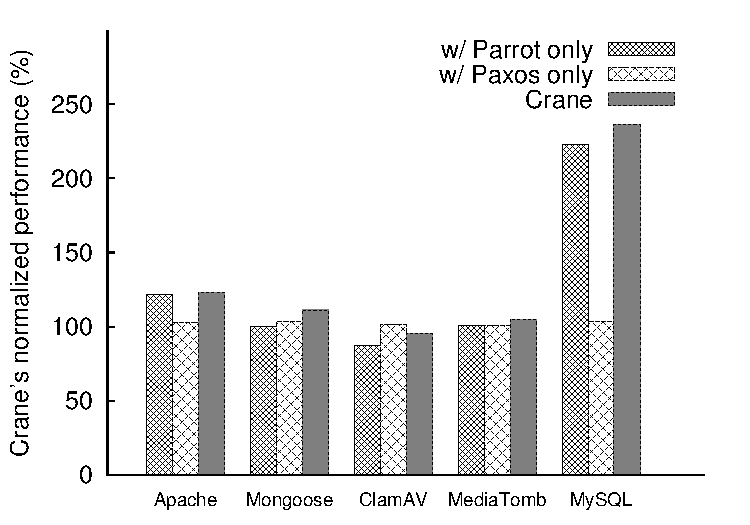
\includegraphics[width=0.5\textwidth]{figures/normalize-perf}
\vspace{-.10in}
\caption{\small {\em \xxx's performance normalized to un-replicated 
nondeterministic execution.}}
\label{fig:normalize-perf}
\end{figure}

% \begin{table}[b]
% \footnotesize
% \centering
% \vspace{-.05in}
% \begin{tabular}{lrrr}
% {\bf Program} & {\bf Percentage (\%)} \\
% \hline\\[-2.3ex]
% \apache                       & 1.14        \\
% \mongoose                       & 3.03        \\
% \clamav                                   & 20.96     \\
% \mediatomb                       & 23.76        \\
% \end{tabular}
% \vspace{-.05in}
% \caption{{\em Percentage of inserted time bubbles among all consensus 
% requests.}} 
% \label{tab:bubble-percentage}
% \end{table}

To understand the performance impact of \xxx's components, we divided \xxx's 
components into two major parts: the \dmt part ran by \parrot; and the proxy 
(with \paxos) part which enforces the same sequence of client socket 
calls across replicas. Each part ran independently without the other 
part. The proxy part represents the performance overhead of invoking \paxos 
consensus for client socket calls, and the \dmt part represents the \parrot 
\dmt scheduler's overhead.

Figure~\ref{fig:normalize-perf} shows the servers' performance running in 
\xxx normalized by their un-replicated nondeterministic executions. The mean 
overhead of \xxx for the \nprog evaluated programs is \overhead 
due to two main reasons. First, except for \mysql, which does fine-grained, 
per-table mutex and read-write locks frequently, the \dmt schedules were 
efficient on the other four servers. The reason is that \parrot's scheduling 
primitives are already highly optimized for multi-core~\cite{parrot:sosp13}. 
The proxy-only part incurred 0.82\%$\sim$3.46\% overhead, which is not 
surprising, because the number of socket calls is much smaller than 
the number of \pthread synchronizations in these programs. In short, \xxx's 
performance mainly depends on the \dmt schedules' performance.

\mediatomb incurred modest speedup because its transcoder \mencoder had 
significant speedup with \parrot. We inspected \mediatomb's micro performance 
counters with the Intel \vtune~\cite{vtune} profiling tool. When running in 
\xxx, \mediatomb only made 6.6K synchronization context switches, while in the 
\pthread runtime it made 0.9M synchronization context switches. This saving 
caused \mediatomb running with \parrot a 12.76\% speedup compared 
to its nondeterministic execution. The \parrot evaluation~\cite{parrot:sosp13} 
also observed a \mencoderspeedup speedup on the \mencoder program. 

The \timealgo technique saves most of needs on invoking consensus 
for the logical times of clients' socket operations, confirmed by the low 
frequency of inserted time bubbles in Table~\ref{tab:timebubbles}. \apache, 
\mediatomb, and \mongoose uses \ab as its benchmark, and each request contained 
a \connect, \send, and \close call. \clamav uses its own \v{clamdscan} 
benchmark, and each request contained 18 socket calls. \mysql's benchmark 
contained 6$\sim$7 socket calls for each query. The ratio of inserted 
bubbles is merely 6.12\%$\sim$33.35\%. \mediatomb had the highest ratio of time 
bubbles because it took the longest time (9,703ms) to process each 
request.

Note that the number of inserted time bubbles across replicas is the 
same within the same run of \xxx. Within different runs of \xxx, this number 
can be different because \ntimeout is a physical duration.

\begin{table}[b]
\footnotesize
\centering
\vspace{-.05in}
\begin{tabular}{lrrr}
{\bf Program} & {\bf \# client socket calls} & {\bf \# time bubbles}  & {\bf 
\%} \\
\hline\\[-2.3ex]
\apache                       & 3,000        &    450 &    13.04 \\
\clamav                                   & 18,000     &    1,173 &    6.12 \\
\mediatomb                       & 3,000        &    1,501 &    33.35 \\
\mongoose                       & 3,000        &    448 &    12.99 \\
\mysql                       & 6,750        &    573 &    7.82 \\
\end{tabular}
\vspace{-.05in}
\caption{{\em Ratio of time bubbles in all \paxos consensus 
requests.}} 
\label{tab:timebubbles}
\end{table}

\subsection{Optimization of \parrot's Performance Hints} \label{sec:hint}

\begin{figure}[t]
\centering
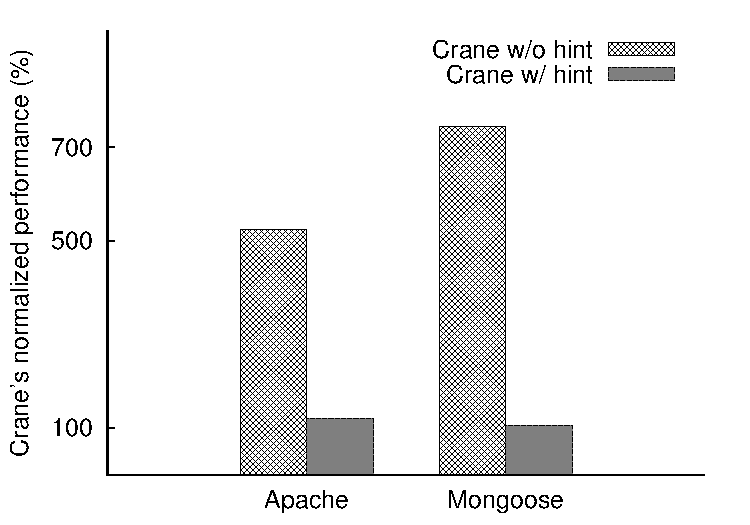
\includegraphics[width=0.5\textwidth]{figures/opt-hint}
\vspace{-.10in}
\caption{\small {Effects of \parrot's soft barrier performance hints.}}
\label{fig:opt-hint}
\end{figure}

In general, a \dmt schedule may be slow in some cases~\cite{parrot:sosp13, 
dthreads:sosp11}, because this schedule may \emph{serialize} some major 
computations that can run in parallel in the \pthread runtime. For instance, 
when we ran \xxx's \dmt scheduler \parrot with \apache and \mongoose, we 
observed that \parrot's default schedules serialized the PHP interpreters.

Fortunately, \parrot creates a set of easy to use, intuitive soft barrier 
hints~\cite{parrot:sosp13} which tell the \dmt runtime to switch to faster 
schedules. These hints are just ``soft" barriers; they timeout 
deterministically and can tolerate different number of concurrent incoming 
requests. They just make a (deterministic) effort to line up computations that 
tend to run in parallel. In addition, these hints can be safely ignored by the 
\parrot runtime without affecting a program's logic.

In our evaluation, we added two lines of hints for each of the \apache and 
\mongoose servers' source code, and the pattern was general: one line was 
added at the server's \v{main()} function to initialize the soft barrier, and 
the other before a PHP interpretation's start to tell the \dmt scheduler 
``these are the major computations to line up". The performance optimization 
effects of these hints are shown in Figure~\ref{fig:opt-hint}. These hints 
reduces \apache's overhead from a 424\% to 22.99\%, and \mongoose's from a 643\% 
to 5.09\%.

% In our evaluation, we added two lines of hints for each of the \apache and 
% \mongoose programs. The methodology of adding hints to these server programs 
% are similar: one line \v{soft\_barrier\_init(0,} \v{maxworkers,} 
% \v{100*maxworkers)} was added in the server's \v{main()} function to initialize 
% a soft barrier with an opaque id 0, and the estimated number of max worker 
% threads, and also the number of logical clock ``100" that each thread need to 
% wait on this soft barrier to line up with other threads. In our evaluation, the 
% \v{maxworkers} is the 8, the number of threads with peak performance of these 
% servers running on our machines. The second line \v{soft\_barrier\_wait(0);} 
% was 
% added before a worker thread starts to process a \http request, so that threads 
% can line up at this point with the other threads with the same opaque id and 
% process requests in parallel. These hints are just ``soft" barriers; 
% they timeout deterministically and can tolerate different number of concurrent 
% incoming requests; they just make a (deterministic) effort to line up 
% computations that tend to run in parallel.



\subsection{Sensitivity of Time Bubble Parameters} \label{sec:sensitivity}
\begin{figure}[t]
\centering
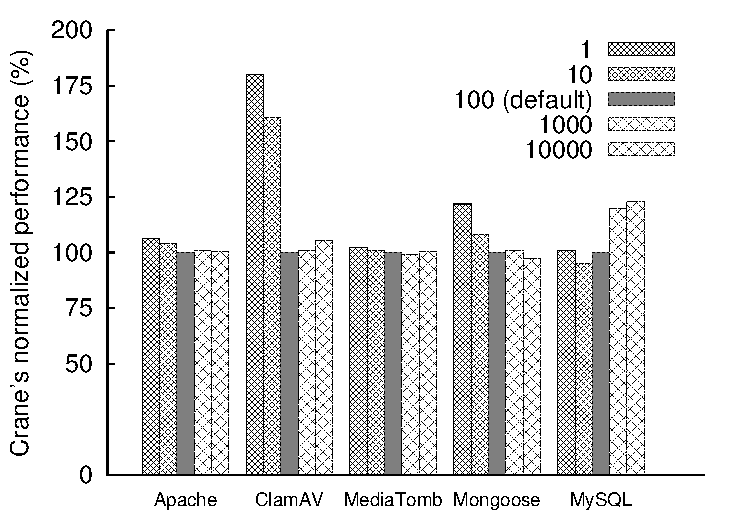
\includegraphics[width=0.5\textwidth]{figures/usleep-sensitivity}
\vspace{-.10in}
\caption{\small {\em \xxx's performance with different settings on \ntimeout 
(us).} Normalized with the default parameter.}
\label{fig:usleep-sensitivity}
\end{figure}

\begin{figure}[t]
\centering
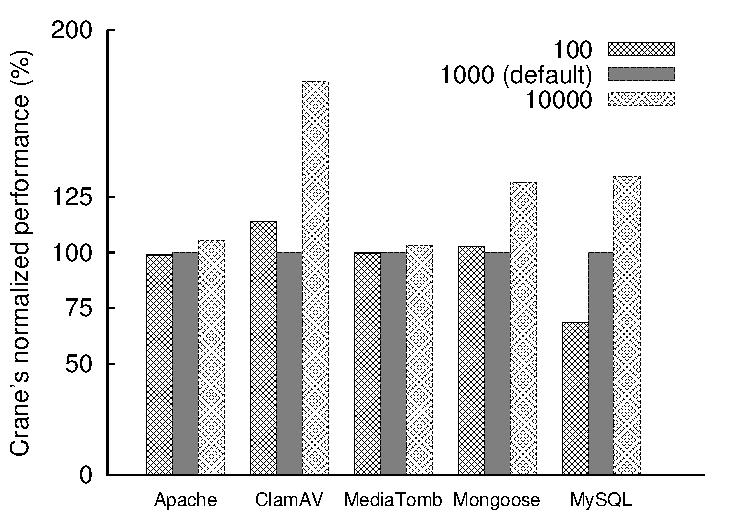
\includegraphics[width=0.5\textwidth]{figures/nclock-sensitivity}
\vspace{-.10in}
\caption{\small {\em \xxx's performance with different settings on \nclock.} 
Normalized with the default parameter.}
\label{fig:nclock-sensitivity}
\end{figure}

The two parameters \ntimeout and \nclock for \timealgo have trade-off on 
performance. This trade-off also depends on each server program as well as its 
performance workload. A smaller \ntimeout means the \dmt 
scheduler can wait less time and then proceed with granted logical clocks with 
inserted time bubbles, but it also means that more time bubbles and thus more 
\paxos consensus are involved. A smaller value also means \timealgo runs 
similar to a per-request consensus approach. 
Figure~\ref{fig:usleep-sensitivity} shows \xxx's performance by only adjusting 
this parameter. \xxx's default setting got the best result for both \apache 
and \clamav, and it got the second best result for the other three programs. 

The \nclock parameter also faces trade-off on performance. A smaller value 
means that servers can exhaust clocks in a time bubble sooner, but if a server 
does lots of \pthread synchronizations to process a request, more time bubbles 
and thus more \paxos consensus are involved. 
Figure~\ref{fig:nclock-sensitivity} shows \xxx's performance by only adjusting 
this parameter. \xxx's default setting got the best result for \clamav, 
\mediatomb, and \mongoose, and the second best result for the other two 
programs.



\subsection{Checkpoint and Recovery} \label{sec:recovery}

\begin{table}[b]
\footnotesize
\centering
\vspace{-.05in}
\begin{tabular}{lrrrr}
{\bf Program} & {\bf C p (ms)} & {\bf R p (ms)} & {\bf C fs (ms)}  & {\bf R fs 
(ms)}\\
\hline\\[-2.3ex]
\apache                       & 33  & 48        &    3,069  & 237 \\
\clamav                               & 415  & 353     &    6,963  & 6,128 \\
\mediatomb                       & 17  & 27        &    2,852  & 213 \\
\mongoose                       & 15  & 31        &    1,294  & 169 \\
\mysql                       & 88  &  81       &    53,473  & 712 \\
\end{tabular}
\vspace{-.05in}
\caption{{\em Average time cost for \xxx's checkpoint and restoring 
component.} ``C p" means ``Checkpoint process", ``R p" means ``Restore 
process", ``C fs" means ``Checkpoint file system", and ``R fs" means 
``Restore file system".} 
\label{tab:checkpoint-time}
\end{table}

To handle replica failures, \xxx periodically invokes a checkpoint operation on 
one backup. Each \xxx checkpoint operation 
contains four time consuming parts: (1) using \criu to dump the state of a 
server process (and its child processes, if any); (2) stopping and restarting a 
\lxc container; (3) doing an incremental checkpoint on a server's current 
working directory and installation directory between the \lxc stop and start; 
and (4) restoring a process's state after the \lxc restart.

Table~\ref{tab:checkpoint-time} shows time costs for each process and file 
system checkpoint operation, and all are median values with 
20 runs. In sum, a process checkpoint or restore took at most 415ms, and a file 
system checkpoint or restore took less than 7s except \mysql. \mysql took about 
one minute to checkpoint its file system because \sysbench generated a large 
database in \mysql's installation directory. For each program, a file system 
restore operation took much less time than its checkpoint operation because a 
restore 
operation patches only files modified by the server program. A common \lxc stop 
and restart operation took 2$\sim$5s depending on the daemon processes' 
bootstrap progress within the container. Although each of these four steps in a 
\xxx checkpoint operation costs time, such a checkpoint is done on only one 
backup replica, its performance impact was negligible in our evaluation (the 
other replicas formed a quorum).

To evaluate the speed of \xxx's \paxos protocol on replica failure and 
recovery, we manually restarted the primary replica running a \mongoose server. 
The other two backups in the system then invoked a leader election with three 
steps~\cite{paxos:practical}, which took \recovertime. After 
the old primary's machine restarted, \xxx restarted the proxy and the 
consensus component, extracted the latest \mongoose checkpoint on the local 
machine and restored the \mongoose process and its file system. On the full 
restore of this \xxx instance, it received the new primary's heart beat message 
in \downgradetime and downgraded itself to a backup. Overall, both the \paxos 
leader election and the restarted old primary's self-downgrading took 
sub-seconds.

% We observed that the restored \mongoose server were able to continue to process 
% client requests normally, thanking to \criu and \lxc's robust implementation. 
% Overall, both the leader election and the restarted node's self-downgrading 
% took sub-seconds.



% \section{Related Work} \label{sec:related}
\para{State machine replication (SMR).}  SMR has been studied by the literature 
for decades, and it is recognized by both industry and academia as a powerful 
fault-tolerance technique in clouds and distributed 
systems~\cite{lamportclock,smr:tutorial}. As a common practice, SMR uses 
\paxos~\cite{paxos,paxos:simple,paxos:complex} and its popular engineering 
approaches~\cite{paxos:live,paxos:practical} as the consensus protocol to 
ensure that all replicas see the same input request sequence. Since consensus 
protocols are the core of SMR, a variety of study improve different aspects of 
consensus protocols, including performance~\cite{epaxos:sosp13,paxos:fast} and 
understandability~\cite{raft:usenix14}. Although \xxx's current implementation 
takes a popular engineering approach~\cite{paxos:practical} for practicality, 
it can also leverage other consensus protocols and approaches.


At a system implementation level, \smr typically takes the ``agree-execute" 
approach: replicas first ``agree" on a total order of input request as a input 
sequence, and then ``execute" the requests that have reached this consensus. 
Such typical systems include Chubby~\cite{chubby:osdi}, 
ZooKeeper~\cite{zookeeper}, and the Microsoft \paxos~\cite{paxos} 
implementation, and they have been widely used to maintain critical distributed 
systems configurations (\eg, group leaders, distributed locks, and storage meta 
data). SMR has also been applied broadly to build various highly available 
services, including 
storage~\cite{paxos:datastore,bolosky:nsdi11,spanner:osdi12} and wide-area 
network~\cite{mencius:osdi08}. Hypervisor-based Fault 
Tolerance~\cite{hft:sosp95} leverages a hypervisor to build a primary-back 
system for single-core machines. Unlike \xxx, these systems are not designed to 
transparently replicate general multithreaded server programs. Nevertheless, 
\xxx takes the typical ``agree-execute" approach.


In order to support multi-threading in SMR, Eve~\cite{eve:osdi12} introduces a 
new ``execute-verify" approach: it first executes a batch of requests 
speculatively, and then verifies whether these requests have conflicts that 
cause execution state divergence. If so, Eve rolls back the program to a state 
before executing these requests and re-execute these requests sequentially. 
Both Eve's execution divergence verification and rollbacks require developers 
to manually annotate all shared states, which is time consuming and 
error-prone. 

Rex~\cite{rex:eurosys14} addresses the thread interleaving divergence problem 
with a ``execute-agree-follow" approach: it first records thread interleavings 
on the primary by executing requests, and then replays these interleavings 
on the other backups. If the executed interleavings in the primary may not be 
agreed on the other replicas, then Rex rollbacks the primary's states. These 
rollbacks/checkpoints also require developers' manual efforts for every 
program. Furthermore, Rex requires frequently shipping thread interleavings 
across replicas, which may be slow. Unlike \xxx's transparent 
checkpoint-restore mechanism, Rex requires program developers to implement 
the checkpoint-restore logic.

To improve performance, some \smr systems~\cite{eve:osdi12, pbft:osdi99, 
upright:sosp09, zyzzyva:sosp07, zookeeper} perform read-only optimization 
on request interface and allow these requests to be processed rapidly without 
consensus. \xxx currently does not explore this direction mainly for two 
reasons. First, \xxx's performance overhead is already moderate in our 
evaluation. Second, some read requests may still modify programs' internal 
execution states (\eg, \apache's internal HTTP cache) and affect outputs. Thus,
ensuring whether a request is indeed read-only for a general server program may 
require understanding or crafting the program significantly, which may trade 
off transparency. However, exploring the trade-off between \xxx's transparency 
and performance is an interesting direction.

\para{\dmt and \smt systems.}  In order to make multi-threading easier to 
understand, test, analyze, and replicate, researchers have built two types of 
reliable multi-threading systems: (1) stable multi-threading systems (or 
\smt)~\cite{grace:oopsla09, dthreads:sosp11, determinator:osdi10} that aim to 
reduce the number of possible thread interleavings for program all inputs, and 
(2) deterministic multi-threading systems (or \dmt)~\cite{dpj:oopsla09, 
dmp:asplos09,kendo:asplos09,coredet:asplos10,dos:osdi10,ddos:asplos13,
ics:oopsla13} that aim to reduce the number of possible thread interleavings on 
each program input. Typically, these systems use deterministic logical clocks 
instead of nondeterministic physical clocks to make sure inter-thread 
communications (\eg, \mutexlock and accesses to global variables) can only 
happen at some specific logical clocks. Therefore, given the same or similar 
inputs, these systems can enforce the same thread interleavings and eventually 
the same executions. These systems 
have shown to greatly improve software reliability, including coverage of 
testing inputs~\cite{ics:oopsla13} and speed of recording 
executions\cite{dos:osdi10} for debugging.

Typical DMT systems, including \kendo~\cite{kendo:asplos09}, 
\coredet~\cite{coredet:asplos10}, and \coredet-related 
systems~\cite{dos:osdi10, ddos:asplos13}, improve performance by balancing each 
thread's load with low-level instruction counts, so they are unstable to 
input perturbations. \ddos~\cite{ddos:asplos13} demonstrates that a distributed 
system can be made deterministic. However, our \xxx approach is more flexible, 
because we can choose to focus on replicating servers' execution states only 
and discard clients' states, then \xxx has fewer scheduling constraints and can 
be more efficient.



% %% First introduce checkpoint techniques that do not support threads.
% \para{Checkpointing program states.} Checkpointing is a common technique in 
% systems with critical fault-tolerance demands, and the specific checkpoint 
% requirements depend on the target system design. In the last few decades, 
% checkpointing distributed systems~\cite{beguelin:jpdc97, dejavu:ipdps07, 
% dmtcp:ipdps09, oren:atc07} is well studied. Our \xxx system uses 
% \criu~\cite{criu}, a robust, open source checkpoint-restore tool to build our 
% transparent checkpoint-restore service. \xxx carefully selects a good 
% checkpoint timing~\ref{sec:checkpoint} to avoid the tedious effort on 
% checkpointing and restoring network stack.
% 
% %% Introduce techniques that support threads.
% Recently, checkpointing threads on multi-core is studied in a debugging 
% technique called deterministic 
% replay~\cite{smp-revirt:vee08,pres:sosp09,odr:sosp09,scribe:sigmetrics10,
% capo:asplos09}. For instance, SMP-ReVirt~\cite{smp-revirt:vee08} and 
% Scribe~\cite{scribe:sigmetrics10} use clever page protection tricks to record 
% memory accesses. Unfortunately, these checkpoint techniques do not meet 
% \xxx's 
% purpose, because the replayed executions in these systems are mainly for 
% debugging and don't need to go live (\eg, the network sockets and file 
% descriptors are normally fake). However, our \xxx system requires that 
% the checkpointed executions must be live on remote nodes and can serve 
% future requests.

\para{Concurrency.} \xxx are mutually beneficial with much prior work on 
concurrency error 
detection~\cite{yu:racetrack:sosp,savage:eraser,racerx:sosp03,lu:muvi:sosp,
avio:asplos06,conmem:asplos10},
diagnosis~\cite{racefuzzer:pldi08,ctrigger:asplos09,atomfuzzer:fse08}, and
correction~\cite{dimmunix:osdi08,gadara:osdi08,wu:loom:osdi10,cfix:osdi12}. 
On one hand, these techniques can be deployed in \xxx's backups and help 
\xxx detect data races. On the other hand, \xxx's asynchronous replication 
architecture can mitigate the performance overhead of these powerful 
analyses~\cite{repframe:apsys15}.

% 
% common weaknesses of Rex, ddos and dos: 
%   - per-request consensus on schedule or logical time
%   - no checkpoint and recovery

\section{Conclusion} \label{sec:conclusion}
We have presented \xxx, a \smr system that 
transparently replicates general server programs without 
requiring server developers' intervention. It provides a new state machine 
interface compatible to socket API, and it leverages 
deterministic multithreading to enforce the same schedules for a multithreaded 
server program across replicas. \xxx creates a \timealgo technique to 
efficiently enforce consistent logical times on admitting network requests 
across replicas.

Evaluation on \nprog widely used server programs shows that 
\xxx is easy to use, has moderate overhead, and provides practical recovery 
support. \xxx has the potential to expand the adoption of \smr and to provide 
transparent fault-tolerance support for general server programs. \xxx's 
source code is at \github.

% \section*{Acknowledgments}

We thank Marcos K. Aguilera (our shepherd), Yinzhi Cao, Adrian Tang, David 
Williams-King, and anonymous reviewers for their many helpful comments. This 
work was supported in part by AFRL FA8650-11-C-7190 and FA8750-10-2-0253; ONR 
N00014-12-1-0166; NSF CCF-1162021, CNS-1054906; an NSF CAREER award; an AFOSR 
YIP award; and a Sloan Research Fellowship.


\end{sloppypar}

% uncomment to tweak with bib spacing
%\setlength\bibsep{2.25pt}
{
%\small
 \bibliographystyle{abbrvnat}
 \bibliography{bib/biblio}
}

\end{document}
